\section{Architecture}
%
This section introduces the architecture of the currently distributed version of PostgreSQL.
%
Furthermore it is shown how the architecture looks after the refactoring and implementation of the new algorithm.
%
\subsection{Current architecture}
%
In the current version of PostgreSQL the access control module is not identifiable as own module in the backend code of the DBMS.
%
The following figure shows a flowchart of the backend of PostgreSQL.
%
It is shown that there are two general types of queries: \emph{utility commands} and \emph{non-utility commands}.
%
Utility commands include all commands that modify the structure of the database, i.e., add a new table or view, create a trigger, or modify ACLs for example.
%
Non-utility commands on the other hand, modify the data in the underlying database structure, i.e., add tuples, update tuples or delete tuples for example.
%
The main difference between those is that the utility commands are generally \emph{non-optimizable}.
%
That means it makes no sense to pass them through the query rewriter or optimizer, since there is generally no room for optmization.
%
Non-utility commands however are passed through several stages of the backend, where they are rewritten, plans are generated, the optimal plan is chosen and finally the optimal plan is executed.
%
As mentioned before there is no interface that allows these different stages of the backend to request a access control decision.
%
Therefore the decision if a query is authorized or not is usually done inside the so called traffic cop, which, as the name indicates, moderates the incoming queries to the correct modules.
%
Inside the traffic cop however it depends again on the exact type of the query, i.e., if the query is a \texttt{SELECT}, \texttt{INSERT} or other type, how the decision is made.
%
Due to this the access control mechanism in the current version of PostgreSQL is deeply connected with the internals of the backend, because the functions usually do not only retrieve the ACL, but prepare the system catalogs, the tables that contain the database structure, for the upcoming change.
%
Sometimes however, such as in the case of a \texttt{CREATE TRIGGER} command, the decision is made in the course of creating the trigger, i.e., there is no external function called that makes the decision.
%
\begin{figure}[!ht]
  \centering
    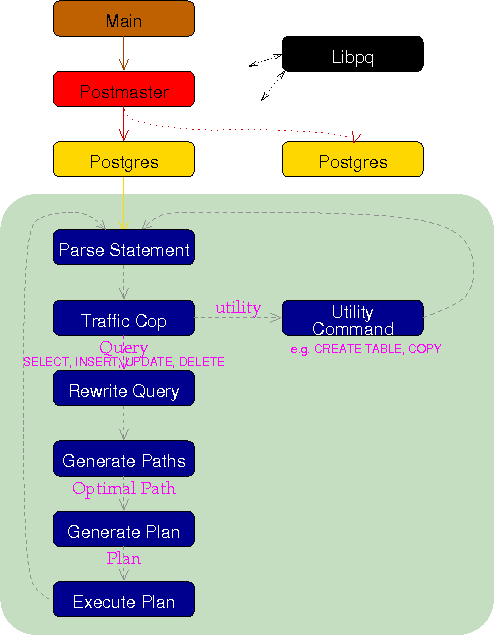
\includegraphics[width=1\textwidth]{img/backend_flowchart.png}
    \caption{Backend Flowchart PostgreSQL \protect \footnotemark}
\end{figure}
%
\footnotetext{\url{http://www.postgresql.org/developer/backend}}
%
\FloatBarrier
%
\subsection{Refactoring}
%
After analyzing the backend, by executing each type of query and following the backend throught the process with a debugger, all the functions or code regions relevant to making access control decisions was identified.
%
This identification allowed to gradually move the code to a external module and build a uniform interface which is called inside the traffic cop, when the backend expects a decision.
%
The building of a uniform interface however introduced several engineering challenges.
%
Depending on the function the type of the return value is different. Also some code that was moved to the external module was not a function, but part of a function without a return value.
%
\remark{I find it difficult to add more content here, should I describe specific examples? It is the thing that took most of the time...}
%
After the process of refactoring it is possible to integrate any access control mechanism as a plug-in.
%

%
\subsection{Implementation}